\clearpage
Blank
\clearpage

\section{Introduction}

\subsection{Motivation}

In the age of digital documents, an author of content is confronted with the
question which document format to choose. Since every document format has its
advantages, one might not want to commit to a specific format to soon.

A series of blog posts might turn into a book or at least a pretty typeset
\emph{pdf}. An author also might want to give the reader the freedom to read
their text on different digital devices—e.g. mobile phones, tablets and e-readers.

Luckily the problem of decoupling the initial document from output seems to be
solved by the rise of markup languages such as Markdown and the like. These
types of documents can be easily compiled into all sorts of output formats by
programs such as \emph{Pandoc} \cite{pandoc}.

If the reader has no objections to such a publishing system, they might read no
further and write away their next \emph{format-agnostic} document. But if they
are interested in how they can easily extend the representation of their
document and let a type-checker reason about the \emph{well-formedness} of it,
they may find the findings gathered in this paper worth while.

\subsection{Type-safe extensibility}

This paper mostly outlines the ideas of the work on \emph{HSXML: Typed SXML}
\cite{hsxml} and its underlying approach of \emph{tagless-final style}
\cite{finally-tagless, finally-tagless-tut}.\\
The \emph{tagless-final style} is a solution to the expression problem
\cite{expression-problem}. It is closely related to the problem at hand, in that
it is concerned with the simultaneous extension of syntactic \emph{constructors} and
interpretations of them—we call those \emph{observations}. This can be seen as an
extensibility in two dimensions. For those unfamiliar with the the expression
problem—section \ref{section_ep} provides a short introduction.

\subsection{?}

In short a \emph{tagless-final encoded} representation of documents like
\emph{HSXML} has in our opinion two major advantages over markup languages such
as Pandoc’s internal one:

\begin{enumerate}
\item Guarantee the well-formedness of the document by construction
\item Easy and full extensibility without loosing the guarantees of 1.
\end{enumerate}

While having these two advantages we still do not want to loose perspective and
solve to our initial goal:

\begin{enumerate}
\item Writing documents that are format agnostic—i.e. observe our source in
different ways
\end{enumerate}

or as described in the Wikipedia-article on \emph{Markup Languages}

\begin{quote}
Descriptive markup

Markup is used to label parts of the document rather than to provide specific
instructions as to how they should be processed. Well-known examples include
\LaTeX{}, HTML, and XML. The objective is to decouple the inherent structure of
the document from any particular treatment or rendition of it. Such markup is
often described as "semantic".
\end{quote}

\clearpage

\section{Background: The Expression Problem} \label{section_ep}

The following description of the expression problem is short and precise and
stems from Zenger’s and Odersky’s paper \emph{Indepently Extensible Solutions to
  the Expression Problem} \cite{indie_solutions}.

\begin{quote}
  Since software evolves over time, it is essential for software systems to be
  extensible. But the development of extensible software poses many design and
  implementation problems, especially if extensions cannot be anticipated. The
  \emph{expression problem} is probably the most fundamental one among these
  problems. It arises when recursively defined datatypes and operations on
  these types have to be extended simultaneously.
\end{quote}

In this paper we call those \say{datatypes} \say{data variants} or short
\say{variants} and the operations on them are called \say{observations}. This is
inspired by \emph{Extensibility for the Masses} \cite{object_algebra}.

To get a better intuition on what the expression problem is really concerned
with, we will introduce a small extensibility problem and explain the meaning of
these \emph{mystical dimensions} with its help:

The task is to find an easily extensible representation of \emph{algebraic
  expressions}—like e.g. $2+4-3$—in Haskell. We will present three different
encodings and discuss what kinds of extensibility they allow.

\subsection{ADT encoding}

When encoding algebraic expressions in \emph{algebraic data type (ADT)
  encoding}, we could write this definition:

\begin{lstlisting}
data Expr
  = Lit Int
  | Add Expr Expr
\end{lstlisting}

With the above code we defined two data variants—\texttt{Lit} and
\texttt{Add}—and now we can write multiple observations on those variants
easily:

\begin{lstlisting} 
eval :: Expr -> Int
eval (Lit i)   = i
eval (Add l r) = eval l + eval r

pretty :: Expr -> String
pretty (Lit i)   = show i
pretty (Add l r) =
     "(" ++ pretty l ++ ")"
  ++ "+"
  ++ "(" ++ pretty r ++ ")"
\end{lstlisting}

We assess that the ADT encoding is extensible in the dimension of observations.

If we wanted to add another variant—e.g. one for negation—we would have to
change not only the ADT definition but also all observations. This might be
feasible as long as we feel comfortable with changing the original code. But as
soon as someone else wrote observations depending on the original set of
variants, we risk breaking compatibility.

\subsection{OO encoding}
If we wanted to ensure that our representation is extensible in the dimension of
data variants, we could choose the \emph{object oriented (OO) encoding}. This
encoding is centered around the record type \texttt{ExprOO} with the following
definition:
\begin{lstlisting}
data ExprOO = Expr { evalThis :: Int
                   , prettyThis :: String}
\end{lstlisting}

This definition states: an \texttt{Expr} is a value that can be evaluated to
both an \texttt{Int} and a \texttt{String}. Based on this we can create a set of
constructors.

\begin{lstlisting}
newLit :: Int -> ExprOO
newLit i = Expr i (show i)

newAdd :: ExprOO -> ExprOO -> ExprOO
newAdd l r = Expr evalResult prettyResult
 where
  evalResult   = evalThis l + evalThis r
  prettyResult =
       "(" ++ prettyThis l ++ ")"
    ++ "+"
    ++ "(" ++ prettyThis r ++ ")"
\end{lstlisting}

This set of data variants can now be easily extended. In the following we define
a constructor representing the algebraic operation of \emph{negation}.

\begin{lstlisting}
newNeg :: ExprOO -> ExprOO
newNeg e = Expr (- evalThis e) ("- " ++ prettyThis e)
\end{lstlisting}

These constructors can be used like the constructors of the ADT encoding to
create ASTs.

\begin{lstlisting}
exOO :: ExprOO
exOO = newAdd (newLit 4) (newNeg (newLit 2))
\end{lstlisting}
\begin{lstlisting}
> evalThis exOO
2
\end{lstlisting}

Although this representation is extensible in the dimension of data variants,
the set of observations is fixed by the definition of the \texttt{ExprOO} type.

\subsection{Church/Böhm-Berarducci encoding}
\label{subsection_BB_encoding}

Finally we will choose \emph{Böhm-Berarducci (BB) encoding} for our
representation which is the foundation of the tagless-final style.

Böhm and Berarducci used a technique, that is similar to Church
encoding, to show that ADTs can be represented by using solely using function
application and abstraction in \emph{System F} (i.e. polymorphic
lambda-calculus) \cite{boehm_berarducci}.

In practice this means that we could define lists, instead of using an ADT, the
following way:

\begin{lstlisting}
bbList :: (Int -> a -> a) -> a -> a
bbList cons nil = cons 2 (cons 1 nil)
\end{lstlisting}

To paraphrase the code: if we are supplied one interpretation for the
\texttt{nil} variant and one interpretation for the \texttt{cons} variant—that
takes one \texttt{Int} and the already evaluated rest of the list, we can
interpret the whole list.

We can generalize this idea: To evaluate an AST to a type $B$, we need to know
for each node type, how to evaluate it to $B$. If all these needed
\emph{evaluation strategies} are supplied, we can evaluate (i.e. \emph{fold})
the AST from the leaves up. These \emph{evaluation strategies} are called
\textbf{algebras}.\\
This is in essence the idea of Church/Böhm-Berarducci encoding.

In the appendix we include representation that is purely using application and
abstraction for our running example. But in Haskell we are luckily not
restricted to the features of lambda calculus. Therefore we can use record types
for storing \emph{algebras} (i.e. evaluation strategies).

Our algebras are of the following type:

\begin{lstlisting}
data ExprBP a = ExprBP { lit :: Int -> a
                       , add :: (a -> a -> a) }
\end{lstlisting}

The field called \texttt{lit} contains the interpretation for the leaves and
therefore is a function that evaluates an \texttt{Int} to some type \texttt{a}.
The \texttt{add} function takes two evaluated subtrees as an input—in form of
two \texttt{a}—and outputs also a value of type \texttt{a}.

An AST, using this definition, looks like this:

\begin{lstlisting}
exprBP :: ExprBP a -> a
exprBP (ExprBP lit add) = add (lit 4) (lit 2)
\end{lstlisting}

This is analogue to the BB encoded list from before, but, instead of getting
the algebras for \texttt{lit} and \texttt{add} one by one, the AST accepts one
algebra that bundles both.

\subsubsection{Writing algebras}

To evaluate those \emph{BB encoded} algebraic expressions, we have to define
algebras of the type \texttt{ExprBP}:

\begin{lstlisting}
evalExprBP :: ExprBP Int
evalExprBP = ExprBP evalInt evalAdd
  where
    evalInt i   = i
    evalAdd l r = l + r

prettyExprBP :: ExprBP String
prettyExprBP = ExprBP evalInt evalAdd
 where
  evalInt     = show
  evalAdd l r =
       "(" ++ l ++ ")"
    ++ "+"
    ++ "(" ++ r ++ ")"
\end{lstlisting}

\texttt{evalExprBP} can be defined even more concise in Haskell:

\begin{lstlisting}
evalExprBP :: ExprBP Int
evalExprBP = ExprBP id (+)
\end{lstlisting}

The AST from before, \texttt{exprBP}, can now be evaluated by supplying the
wanted algebra:

\begin{lstlisting}
> exprBP evalExprBP
6
> exprBP prettyExprBP
"(4)+(2)"
\end{lstlisting}

We can assess that we could define even more algebras this way and that this
encoding is therefore extensible in the dimension of algebras—i.e. observations.

\subsubsection{Add variants}

We have shown that the BB encoding is extensible in the dimension of
observations/algebras but the open question is how to define new variants.

This is can be done by defining a new data type for constructing algebras:

\begin{lstlisting}
data NegBP a = NegBP { neg :: a -> a }
\end{lstlisting}

Using this data type, we can define two new observations:

\begin{lstlisting}
evalNegBP :: NegBP Int
evalNegBP = NegBP (\e -> -e)

prettyNegBP :: NegBP String
prettyNegBP = NegBP (\e -> "-" ++ e)
\end{lstlisting}

Finally we are able to use \texttt{ExprBP} with \texttt{NegBP} in composition:

\begin{lstlisting}
mixedExpr :: ExprBP a -> NegBP a -> a
mixedExpr (ExprBP lit add) (NegBP neg) = add (lit 4) (neg (lit 2))
\end{lstlisting}
\begin{lstlisting}
> mixedExpr evalExprBP evalNegBP
2
\end{lstlisting}

Therefore the Böhm-Berarducci encoding is extensible in both dimensions.\\
If we wanted to add a new data variant, we would need to add a new data type
definition for creating corresponding algebras. And we can create new observers
by creating values of these data types (i.e. algebras).\\
As we have shown, these extensions also compose quite well in BB encoding. [Add
something about Odersky’s paper]

Those familiar with the \say{Scrap your Boilerplate} [add citation] pattern
might notice that the \texttt{ExprBP} data type could also be defined as a type
class and the algebras—\texttt{evalExprBP} and \texttt{prettyExprBP}—as
instances of this type class. In section \ref{section_tagless-final} we will
demonstrate how the encoding with type classes looks like.

%(Figure \ref{Expression_Problem})
%
%\vspace*{\fill}
%\begin{figure}
%    \centering
%    \includegraphics{resources/expression_problem_dimensions.png}
%\captionof{figure}{\label{Expression_Problem}
%Dimensions of the \emph{Expression Problem}}
%\end{figure}
%\vspace*{\fill}
\clearpage

\section{Extensibility of Markup Representations}
\label{main_section}

In the last section we tried to find an extensible representation of
\emph{algebraic expressions} and in this section we will examine how documents
written in markup languages like Markdown or \LaTeX can be represented.

For that reason we will have a look in this section at the representation that
\emph{Pandoc} is using and then show in section \ref{section_tagless-final} how
a representation encoded in tagless-final style is an improvement over that.

\subsection{Extensible Observations}

Pandoc achieves the separation of input and output format by choosing an
algebraic data type (ADT) as its intermediate representation. We will quickly
sketch why such an encoding leads to an easy extensibility of constructors by
looking a subset of Pandoc's abstract syntax tree (AST) and writing some
\emph{observations} for it.

[This paragraph is too short!]
Given the representation (Figure \ref{Pandoc_AST}) we can write observations that
interpret this data in different ways (Figure \ref{Pandoc_Views}). So in the
dimension of observations an ADT encoding is obviously extensible.

Now we can construct a tree in the host language and interpret it in two
different ways:
\begin{lstlisting}
groceryList :: [Block]
groceryList
  = [ Heading 1  [ Str "Grocery list"]
    , BulletList [ Paragraph [ Str "1 Banana"]
                 , Paragraph [ Str "2 "
                             , Emph [Str "organic"]
                             , Str " Apples"]]]

groceryListCM :: Markdown
groceryListCM = mconcatMap docToCMark groceryList

groceryListLaTeX :: LaTeX
groceryListLaTeX = mconcatMap docToLaTeX groceryList
\end{lstlisting}

We can make our life a bit easier by adding an instance for \texttt{IsString}
for our representation. This injects \texttt{String} automatically into our data
types by applying \texttt{fromString} to it.

\begin{lstlisting}
instance IsString Inline where
  fromString = Str
\end{lstlisting}


Our initial definition is now even more concise:

\begin{lstlisting}
groceryListShort :: [Block]
groceryListShort
  = [ Heading 1  [ "Grocery list"]
    , BulletList [ Paragraph ["1 Banana"]
                 , Paragraph ["2 ", Emph ["organic"], " Apples"]]]
\end{lstlisting}

\begin{figure}
\begin{lstlisting}
data Block
  = Paragraph   [Inline] -- ^ Paragraph
  | BulletList  [Block]  -- ^ Bullet list (list of items, each a block)
  | Heading Int [Inline] -- ^ Heading - level (int) and text (inlines)
  
data Inline
  = Str String      -- ^ Text (string)
  | EmDash          -- ^ em dash
  | Emph   [Inline] -- ^ Emphasized text (list of inlines)
  | Strong [Inline] -- ^ Strongly emphasized text (list of inlines)
\end{lstlisting}
\captionof{figure}{\label{Pandoc_AST}
This is part of Pandoc’s ADT-encoded AST modulo \texttt{EmDash}}
\end{figure}

\begin{figure}
\begin{lstlisting}
docToCMark :: Block -> Markdown
docToCMark (Paragraph text)     = mconcatMap inlineToCMark text
docToCMark (BulletList docs)    = ...
docToCMark (Heading level text) = ...

inlineToCMark :: Inline -> Markdown
inlineToCMark (Str content)     = fromString content
inlineToCMARK (Emph contents)   =
            "*"
  `mappend` mconcatMap inlineToCMark contents
  `mappend` "*"
inlineToCMARK (Strong contents) = ...
inlineToCMARK EmDash            = "---"

docToLaTex :: Block -> LaTeX
...

inlineToLaTex :: Inline -> LaTeX
...
\end{lstlisting}
\captionof{figure}{\label{Pandoc_Views}
Observations of ADT encoding}
\end{figure}


\subsection{Extensibility Analysis}

The simple ADT encoding works very well, as long as we have foreseen every
constructor we might want to create. But as soon as we want to add a new kind of
constructor—e.g. a node representing the em dash—we are out of luck. Even if we
have access to the original ADT-definition and we could add this new
constructor, this would break all existing observations that were written for
the original set of constructors.

\subsection{Relationship to the Expression Problem}

[This is now quite redundant. Should kick the whole subsection?]

To be extensible in the dimension of observations as well as the dimension of
the constructors—while still guaranteeing statically their compatibility—is
quite a challenge and one that is common when writing software. It was coined as
the \emph{Expression Problem} by Wadler \cite{expression-problem} and many
solutions have been proposed.

The most prominent solutions—that are widely used the Haskell-ecosystem—are
described in \emph{Data-types a la carte} \cite{data-types-a-la-carte} and in
\emph{Finally Tagless, Partially Evaluated} \cite{finally-tagless}. Kiselyov’s
et al. solution to this is, in our opinion, both easy to use and the notation
for constructing AST is extremely similar to the ADT-encoded one.


\section{Simple Tagless-Final Encoding} \label{section_tagless-final}

Our first attempt to encode our document in the tagless-final encoding will not
have the distinction between \texttt{Doc} and \texttt{Inline}—which was enforced
by the Pandoc-encoding. But later we will see that we are able to recover that
property quite easily with great extensibility properties.

The basic idea of the tagless-final encoding is to create a type class that
specifies all our variants in Böhm-Berarducci encoding. This is analogue to the
\emph{Scrap your type class} variant defined in section
\ref{subsection_BB_encoding}, with the only technical difference:\\
The observers/algebras are now specified with the help of type classes and the
implementations of these specifications are instances of this type class.

\subsection{Böhm-Berarducci encoding with type classes}

In Figure \ref{BB_encoded_AST} we can see that the type classes look basically
like a GADT-encoding where all recursive occurrences and the return-type are
parametrized over.

In contrast to the encoding in section \ref{subsection_BB_encoding}, algebras do
not need to be passed explicitly to the AST definitions. This leads to even more
readable code:

\begin{lstlisting}
groceryList :: (Block a, Inline a) => [a]
groceryList
  = [ heading 1  [str "Grocery list"]
    , bulletList [ paragraph [ str "1 Banana"]]
                 , paragraph [ str "2 "
                             , emph [str "fresh"]
                             , str " Apples"] ]
\end{lstlisting}

The reader might notice that we cannot use the same carrier type for different
interpretations of our AST—otherwise we would get overlapping instances. This
can be quite easily solved by wrapping the carrier type into a \emph{newtype}
and add or derive the needed instances for it. In our case \texttt{Markdown} is
simply a \emph{newtype} of \texttt{String}. Therefore the instances for
\texttt{IsString} and \texttt{Monoid} are straightforward to implement or could
even be derived.

Figure \ref{FT_Observer} shows the implementation of an observer in the
tagless-final encoding. The implementation is really similar the one in the ADT
encoding. But if we have close look, we can see that—since our data type is
Böhm-Berarducci encoded—the observations do not need to be called recursive
explicitly. This makes both our code simpler and is essential for extensibility.

As before, we can automate the injection of \texttt{String} into our encoding by
using the \texttt{OverloadedStrings} language pragma. We do this be adding a
constraint on the type classes, so every output format (i.e. carrier type) must
have an \texttt{IsString} instance.

\begin{figure}
\begin{lstlisting}
newtype Doc doc = Doc doc

-- DocConstraint defined using ConstraintKinds
type DocConstraint doc = (Monoid doc, IsString doc)

instance DocConstraint doc => -- Have to restrict for the use of 'mempty'
  Monoid (Doc doc) where
  mappend (Doc doc1) (Doc doc2) = Doc $ doc1 `mappend` doc2
  mempty = Doc mempty

-- Algebra specification

class Block a where
  paragraph  ::        [Doc a] -> Doc a
  bulletList ::        [Doc a] -> Doc a
  heading    :: Int -> [Doc a] -> Doc a

class DocConstraint a =>
  Inline a where
  emDash ::           Doc a
  str    :: String -> Doc a
  str = Doc . fromString

deleteme $
\end{lstlisting}
\captionof{figure}{\label{BB_encoded_AST}
Böhm-Berarducci encoding using type classes—i.e. tagless-final style}
\end{figure}

\begin{figure}
\begin{lstlisting}
-- Implement Markdown observer

instance Block Markdown where
  paragraph = fromInline . mconcat
  bulletList = ...
  heading level = ...

instance Inline Markdown where
  emDash = "---"

instance Styles Markdown where
  emph   texts = "*"  `mappend` mconcat texts `mappend` "*"
  strong texts = ...


-- Implement LaTeX observer

instance Block LaTeX where
...

instance Inline LaTeX where
...

instance Styles LaTeX where
...
\end{lstlisting}
\captionof{figure}{\label{FT_Observer}
Observer implementation in the tagless-final encoding}
\end{figure}



Interestingly \texttt{Doc} has now no dependency on \texttt{Inline} anymore and
we are now allowed to create the following AST:

\begin{lstlisting}
badHeading = [ heading 1  [ heading 2 [str "Headingception!!"] ] ]
\end{lstlisting}

\clearpage

As noted above, we lost the distinction between \texttt{Doc} and
\texttt{Inline}. But we also gained something—\emph{Doc} can now be used
without \emph{Inline} and we can now also add new constructors without changing our
original constructor definitions:

\begin{lstlisting}
class Styles doc where
  emph   :: [DocWithCtx InlineCtx doc] -> DocWithCtx InlineCtx doc
  strong :: [DocWithCtx InlineCtx doc] -> DocWithCtx InlineCtx doc
\end{lstlisting}

Not only can we now mix those node types at will, but the type of an expression
will reflect which type classes we used for constructing it:

\begin{lstlisting}
stylishNote :: (Inline a, Styles a) => a
stylishNote = strong ["Green Tea keeps me awake"]
\end{lstlisting}

That is why the type system can now statically tell us whether we can evaluate
\texttt{stylishNote} to a particular type.

If we wanted to evaluate an expression that uses constructors that belong to a
type class \emph{X} and evaluate the expression to some carrier type \emph{C},
\emph{C} has to be instance of \emph{X}. Since this is a static property, it can
be decided at compile time.

\subsection{A short note on GHC’s Type Inference}

When we define an AST like \texttt{stylishNote} GHC’s type inference might come
in our way. If no type signature for \texttt{stylishNote} is supplied GHC will
try to infer a concrete type for this definition and not the most generalized
type.

We can avoid this by either supplying the generalized type signature—as done
above—or using the language pragma \emph{NoMonomorphismRestriction}.

\section{Recover Context Awareness}

To regain the context awareness of the Pandoc encoding, we add another field
named \texttt{ctx} to our \texttt{Doc} wrapper (Figure \ref{ContextWrapper}).
\texttt{ctx} is a phantom type and with its help we can specify in which
context a constructor can be used. Since phantom types are not materialized on
the value level, we are simply using empty data declarations as context types.

\begin{lstlisting}
-- Context definitions
data InlineCtx
data BlockCtx
\end{lstlisting}

As shown before, the first tagless-final encoding had the disadvantage, that we
could construct a heading inside another heading. To prohibit this, the
\texttt{heading} constructor has the following context-aware definition:

\begin{lstlisting}
class Block doc where
  heading :: Int -> [DocWithCtx InlineCtx doc] -> DocWithCtx BlockCtx doc
  ...
\end{lstlisting}

The type signature states, that the function expects a
\texttt{DocWithCtx}-wrapper in the \texttt{InlineCtx}-context and returns a
wrapper in the \texttt{BlockCtx}-context. With this refined signature a heading
inside a heading will be rejected by the type system.

To convince Haskell’s type system that a conversion from \texttt{InlineCtx} to
\texttt{BlockCtx} is possible, we can use the following type class:

\begin{lstlisting}
class FromInline ctx where
  fromInline :: DocWithCtx InlineCtx doc -> DocWithCtx ctx doc
  fromInline (DocWithCtx doc) = DocWithCtx doc

instance FromInline BlockCtx
\end{lstlisting}


The set of available contexts should be defined generously, since all
independent extensions of the AST should agree on them. This is obviously are
restriction—but one that is intended.

It is also possible to create context independent constructors. This can be
achieved by parametrizing over the context:

\begin{lstlisting}
class Math doc where
  qed :: DocWithCtx ctx doc
\end{lstlisting}

\begin{figure}[t]
\begin{lstlisting}
newtype DocWithCtx ctx doc = DocWithCtx doc
\end{lstlisting}
\captionof{figure}{\label{ContextWrapper}
Context-aware wrapper}
\end{figure}

\section{Conclusion}

We presented two different encodings that we can choose from for representing a
markup language. While the ADT encoding might look like the tool for the job, we
have seen that it has some serious limitations. Especially if our set of
constructors might scale up and we would do not want to break other people's
observations by changing the ADT definition—the tagless-final approach might be a
good solution also for this instance of the \emph{Expression Problem}.

For those who want to study this approach in more depth—the lecture notes on
\emph{Typed Tagless Final Interpreters} \cite{finally-tagless-tut} are a great
resource.
